\chapter{Data Processing}
\label{chap:data_processing}

Reliable passive face anti-spoofing depends as heavily on dataset hygiene and split isolation as on neural network design. When training data contain unmasked background faces, severe defocus blur, container-format shortcuts, or subject overlap across splits, compact convolutional models rapidly latch onto spurious correlations that collapse during live deployment. This chapter documents the multi-phase self-collected video cohorts, region-of-interest (ROI) extraction rules, optical quality filters, patch representation choices, and person-disjoint validation protocols constructed for this study.

\section{Dataset Description}
\label{sec:dataset_description}

\subsection{General Information}
\label{subsec:dataset_general}

All anti-spoofing and attendance datasets employed in this project are self-collected indoor video corpora acquired under realistic office and classroom illumination. Rather than relying on a single static archive, data collection evolved across three structured cohorts designed to expose and eliminate specific generalization bottlenecks:

\begin{enumerate}
    \item \textbf{Cohort I --- Legacy Webcam Archive (\texttt{dataset/}):} The initial corpus comprises $33$ indoor webcam recordings ($720$p/$1080$p) of bona fide users and handheld screen replay attacks, yielding $24{,}221$ extracted facial crops ($13{,}773$ \texttt{fake} and $10{,}448$ \texttt{real}). Auditing this archive revealed that prior random frame-level splits placed nearly identical consecutive frames into both training and test sets. Re-partitioning the $33$ videos cleanly at the video level established a leakage-free baseline, but subsequent testing on external subjects revealed sharp cross-subject degradation due to limited demographic and presentation diversity.
    \item \textbf{Cohort II --- Multi-Subject Expansion and Merged Multi-Source Benchmark:} To broaden subject diversity, $56$ additional videos ($30$ \texttt{real}, $26$ \texttt{fake}; $1.58$~GB total) were recorded across distinct volunteer identities under varied indoor lighting and mobile display angles. Combining $4{,}925$ unrestricted crops from these $56$ videos with $24{,}032$ quality-verified crops from Cohort~I produced an $89$-video \textbf{Merged Multi-Source Benchmark} ($28{,}957$ crops across two distinct acquisition sources). While invaluable for diagnosing multi-source Batch Normalization drift, diagnostic audits uncovered subtle acquisition confounders between cohorts---most notably QuickTime (\texttt{.mov}) versus MPEG-4 (\texttt{.mp4}) compression characteristics and detector crop-margin differences.
    \item \textbf{Cohort III --- Target-Sensor \texttt{Cam4K} Benchmark (\texttt{dataset\_cam4k/}):} To eliminate cross-container and cross-detector confounding entirely, a dedicated benchmark of $91$ high-definition/4K videos ($44$ \texttt{real}, $47$ \texttt{fake}) was recorded directly on the target deployment sensor: a commercial \textbf{USB SC-M200 camera}. Every recording was stored uniformly in \texttt{.mp4} format and partitioned physically by human subject prior to frame extraction. Scanning $140{,}707$ raw video frames produced $26{,}094$ clean $32\times32$ BGR facial crops ($12{,}618$ \texttt{real}, $13{,}476$ \texttt{fake}). To verify cross-camera retention, an auxiliary external set of $600$ crops ($300$ \texttt{real}, $300$ \texttt{fake}) was captured on an integrated laptop webcam. In parallel, multi-clip bona fide enrollment videos ($2$--$3$ clips per employee) were recorded to calibrate the \texttt{ChamCong\_FaceID} recognition gallery.
\end{enumerate}

\subsection{Statistical Overview}
\label{subsec:dataset_stats}

Table~\ref{tab:dataset_cohorts} summarizes the scale, sensor characteristics, and experimental role of every dataset cohort utilized across the project lifecycle.

\begin{table}[htbp]
\centering
\caption{Overview of video cohorts and evaluation sets used across experimental phases.}
\label{tab:dataset_cohorts}
\small
\begin{tabular}{L{3.5cm}L{2.5cm}R{1.4cm}R{1.8cm}L{4.5cm}}
\toprule
\textbf{Dataset Cohort} & \textbf{Sensor / Format} & \textbf{Videos} & \textbf{Face Crops} & \textbf{Primary Experimental Role} \\
\midrule
Cohort I: Legacy Baseline & USB/Laptop (\texttt{.mp4/\allowbreak.mov}) & $33$ & $24{,}221$ & Expose frame-split leakage; establish clean video-disjoint baseline. \\
\addlinespace[3pt]
Cohort IIa: Quality-Gated Expansion & Multi-device (\texttt{.mov/\allowbreak.mp4}) & $56$ & $7{,}029$ & Multi-subject generalization test \& $12$~s continuous session replay. \\
\addlinespace[3pt]
Cohort IIb: Merged Multi-Source & Dual-source heterogeneous & $89$ & $28{,}957$ & Controlled ablation of BatchNorm drift vs.\ stratified GroupNorm. \\
\addlinespace[3pt]
Cohort III: \texttt{Cam4K} Benchmark & USB SC-M200 (\texttt{.mp4}) & $91$ & $26{,}094$ & Primary person-disjoint training, validation, and unseen test benchmark. \\
\addlinespace[3pt]
External Cross-Cam Set & Integrated Laptop Cam & --- & $600$ & Out-of-domain sensor retention verification ($300$ real, $300$ fake). \\
\bottomrule
\end{tabular}
\end{table}

Because Cohort~III (\texttt{Cam4K}) serves as the definitive production benchmark on target hardware, Table~\ref{tab:cam4k_splits} provides its exact split-level composition extracted from \texttt{extraction\_manifest.json}. Across all three person-disjoint partitions, class priors remain closely balanced ($47.35\%$ \texttt{real} vs.\ $52.65\%$ \texttt{fake} in training; $49.23\%$ \texttt{real} vs.\ $50.77\%$ \texttt{fake} in validation; and $50.84\%$ \texttt{real} vs.\ $49.16\%$ \texttt{fake} in testing), preventing majority-class decision bias.

\begin{table}[htbp]
\centering
\caption{Detailed person-disjoint split statistics of the target-sensor \texttt{Cam4K} dataset ($140{,}707$ raw frames scanned with temporal stride $5$).}
\label{tab:cam4k_splits}
\small
\begin{tabular}{L{2.3cm}R{1.5cm}R{1.5cm}R{1.5cm}R{1.85cm}R{1.85cm}R{1.85cm}}
\toprule
\textbf{Partition} & \textbf{Real Videos} & \textbf{Fake Videos} & \textbf{Total Videos} & \textbf{Real Crops} & \textbf{Fake Crops} & \textbf{Total Crops} \\
\midrule
Training (\texttt{train}) & $30$ & $33$ & $63$ & $7{,}703$ & $8{,}565$ & $16{,}268$ \\
Validation (\texttt{val}) & $7$ & $7$ & $14$ & $2{,}469$ & $2{,}546$ & $5{,}015$ \\
Testing (\texttt{test}) & $7$ & $7$ & $14$ & $2{,}446$ & $2{,}365$ & $4{,}811$ \\
\midrule
\textbf{Total} & $\mathbf{44}$ & $\mathbf{47}$ & $\mathbf{91}$ & $\mathbf{12{,}618}$ & $\mathbf{13{,}476}$ & $\mathbf{26{,}094}$ \\
\bottomrule
\end{tabular}
\end{table}

\subsection{Data Visualization}
\label{subsec:dataset_vis}

Figure~\ref{fig:dataset_samples} displays ten representative $32\times32$ facial crops drawn from the Legacy Webcam and SC-M200 (\texttt{Cam4K}) cohorts, upsampled solely for print legibility. Visual inspection highlights both intra-class diversity (age groups, eyewear, head yaw, and indoor backgrounds) and characteristic presentation attack artifacts: electronic replay crops exhibit elevated high-key screen luminance, subtle chromatic shifts toward blue-magenta display backlights, and reduced micro-shadow contrast along the nasolabial folds compared to bona fide skin.

\begin{figure}[htbp]
\centering
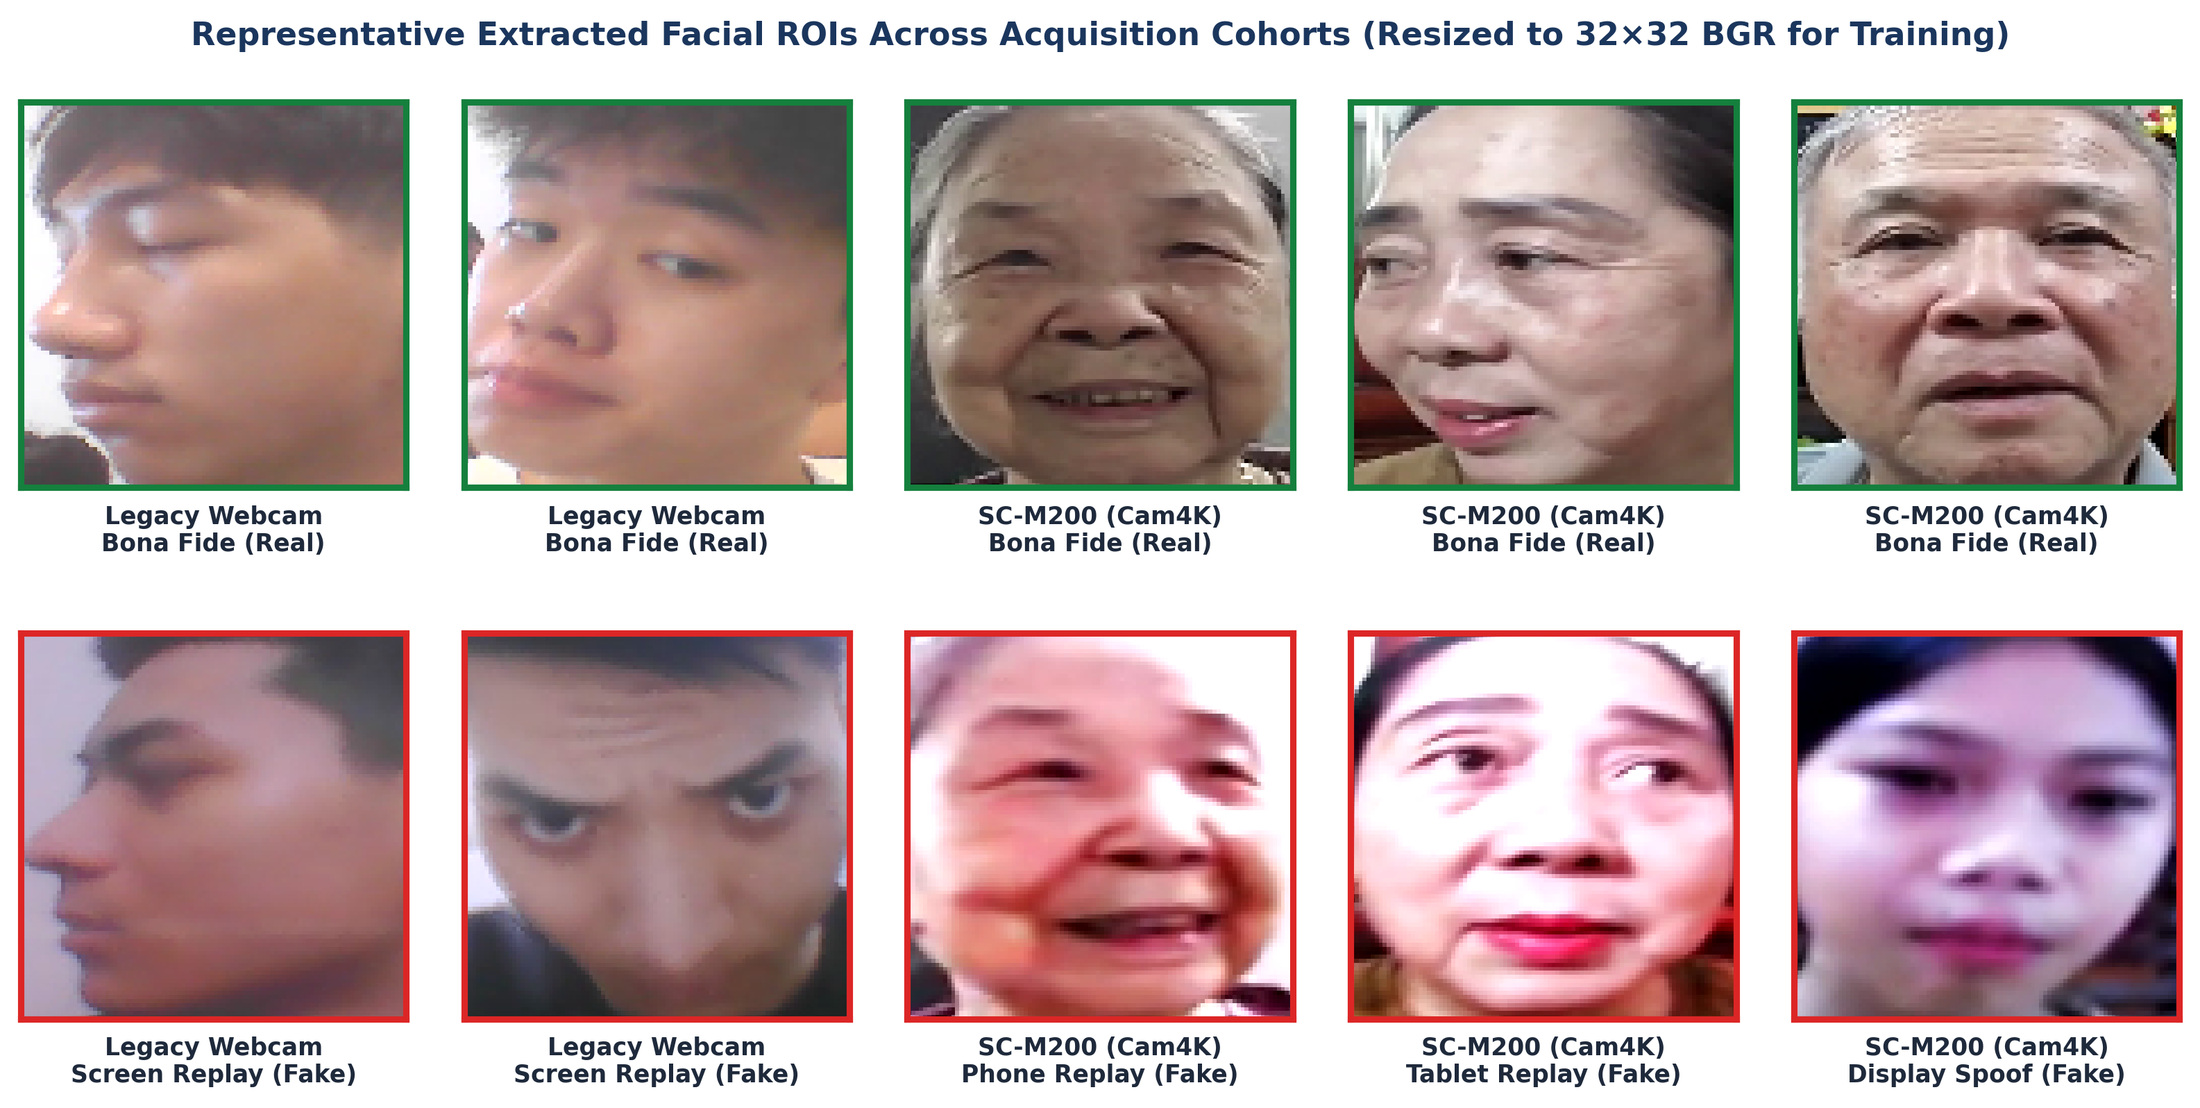
\includegraphics[width=0.96\textwidth]{Images/fig_dataset_samples.jpg}
\caption{Representative extracted facial ROIs across acquisition cohorts resized to $32\times32$ BGR inputs. Top row (green border): bona fide live subjects. Bottom row (red border): smartphone, tablet, and monitor replay attacks.}
\label{fig:dataset_samples}
\end{figure}

Figure~\ref{fig:dataset_statistics} illustrates the structural balance of the \texttt{Cam4K} corpus. Figure~\ref{fig:dataset_statistics}(a) confirms near-parity between bona fide and spoof crops across all three subject-disjoint splits. Figure~\ref{fig:dataset_statistics}(b) plots the per-video crop count distribution across all $91$ videos under temporal stride $5$: both real and fake recordings average $286.7$ extracted crops per video (spanning approximately $55$ to $435$ crops depending on clip duration), motivating video-balanced epoch sampling during training so longer clips do not dominate gradient updates.

\begin{figure}[htbp]
\centering
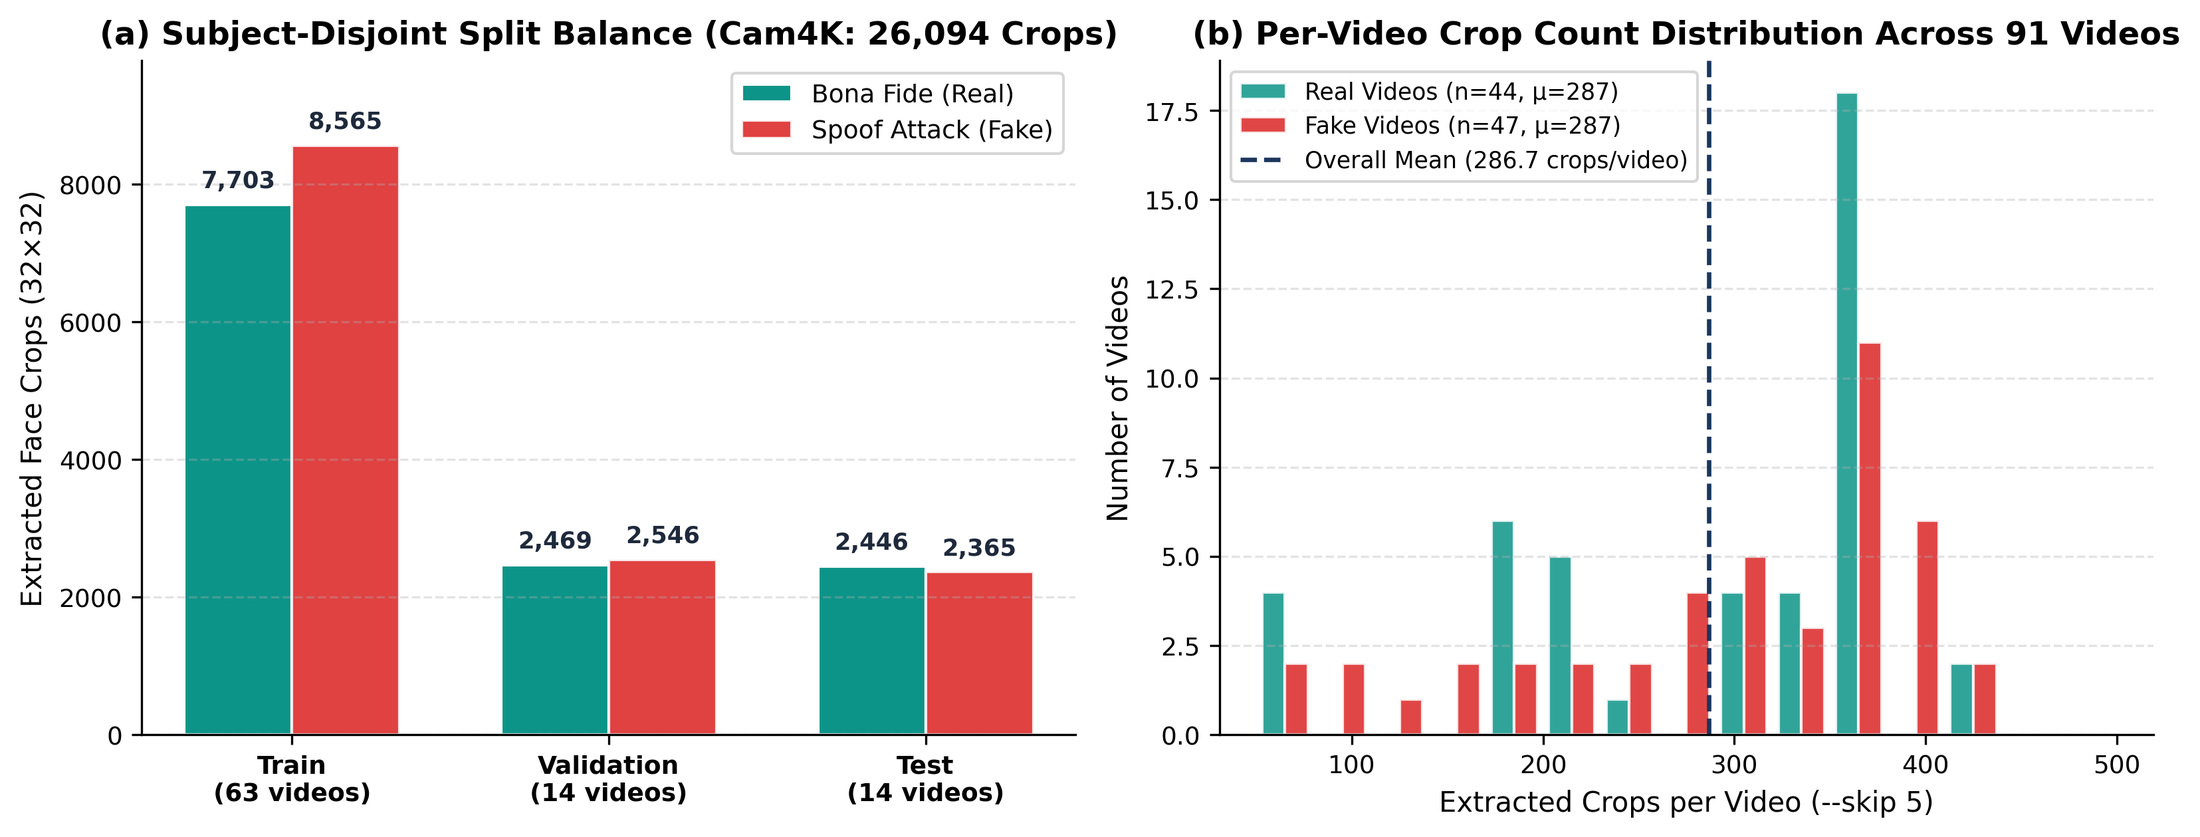
\includegraphics[width=0.98\textwidth]{Images/fig_dataset_statistics.jpg}
\caption{Statistical distribution of the \texttt{Cam4K} benchmark: (a) bona fide versus spoof crop counts across person-disjoint splits; (b) histogram of extracted crops per video across $91$ SC-M200 recordings.}
\label{fig:dataset_statistics}
\end{figure}

\section{Data Preprocessing and Cleaning}
\label{sec:data_preprocessing}

Transforming raw multi-megabyte video streams into clean, supervision-consistent neural network inputs follows a deterministic five-step preprocessing pipeline implemented across \texttt{scripts/extract\_cam4k.py}, \texttt{face\_extract.py}, and \texttt{ChamCong\_FaceID/preprocessing.py}.

\subsection{Temporal Subsampling and Detector Alignment}

Consecutive frames in a $30$~FPS video stream differ minimally in facial pose and illumination. During offline extraction on \texttt{Cam4K}, only every fifth frame (\texttt{--skip 5}, corresponding to $6$~Hz temporal sampling) is evaluated, reducing raw frame volume from $140{,}707$ decoded frames to $26{,}094$ saved crops in $452.6$~seconds while preserving full pose trajectories across each clip. Each sampled frame is resized to $300\times300$, mean-subtracted by $(104.0, 177.0, 123.0)$, and passed through the Caffe ResNet-10 SSD face detector~\cite{liu2016ssd} with confidence threshold $0.50$. When multiple candidate boxes exceed threshold, only the highest-confidence foreground detection with side dimensions $\ge 20$~px is retained.

\subsection{Spatial Masking of Contaminating Presenter Faces}

Manual audit of wide-angle 4K spoof recordings uncovered a subtle label-corruption hazard: in three early attack videos (\texttt{fake\_REC-0001-A.mp4}, \texttt{fake\_REC-0002-A.mp4}, and \texttt{fake\_REC-0003-A.mp4}), the person holding the presentation smartphone stood partially inside the right periphery of the camera field of view. Whenever the smartphone screen tilted momentarily and suffered specular glare, the face detector assigned higher confidence to the live presenter's face on the right edge than to the spoof screen, injecting genuine live faces into the \texttt{fake} training directory. To eliminate this contamination deterministically, \texttt{extract\_cam4k.py} applies a spatial right-edge zero-mask ($I[:, \lfloor 0.65 W \rfloor : W] \leftarrow 0$) prior to face detection on affected wide-angle recordings, guaranteeing that $100\%$ of extracted \texttt{fake} ROIs originate strictly from the attack instrument.

\subsection{Six-Stage Optical Quality Filtering}

During multi-source dataset curation and employee gallery enrollment, raw detections pass through a six-rule optical quality gate grounded in the sharpness formulation of Equation~\eqref{eq:laplacian}~\cite{pech2000diatom}:
\begin{enumerate}
    \item \textbf{Minimum spatial resolution:} Bounding-box width and height must satisfy $\min(w, h) \ge 65$~px for anti-spoofing crops ($\ge 80$~px for ArcFace enrollment) so downsampling does not amplify sensor shot noise.
    \item \textbf{Boundary completeness:} Boxes clipped against frame borders ($x_1 < 0$, $y_1 < 0$, $x_2 > W$, or $y_2 > H$) are discarded to prevent partial-face distortion.
    \item \textbf{Landmark geometry:} When YuNet 5-point keypoints are available, all five landmarks must lie strictly inside the bounding box and the Euclidean inter-ocular distance must satisfy $d_{\text{eye}} \ge 0.12\,w$, filtering extreme profile poses and false background detections.
    \item \textbf{Underexposure floor:} Mean grayscale intensity across the ROI must satisfy $\mu_{\text{gray}} \ge 35$ (on $[0, 255]$) to reject severely shadowed frames where chrominance ratios degenerate into quantization noise.
    \item \textbf{Specular glare ceiling:} The fraction of saturated pixels ($I_{\text{gray}} > 245$) must not exceed $0.45$, preventing washed-out overhead ceiling reflections from masking facial texture.
    \item \textbf{Defocus and motion-blur rejection:} The ROI is standardized to $128\times128$ grayscale so pixel-grid spacing is scale-invariant, and crops with discrete Laplacian variance $\sigma^2_{\text{Lap}} < 12.0$ ($< 45.0$ for high-precision gallery enrollment) are rejected. Applying this audit retroactively to Cohort~I identified and removed $189$ corrupted legacy crops ($158$ excessive glare and $31$ severe motion blur).
\end{enumerate}

\subsection{Normalization, Encoding, and Photometric Augmentation}

Accepted BGR facial crops are bilinearly resized to $32\times32\times3$ and linearly normalized to floating-point $[0, 1]$ by dividing pixel intensities by $255.0$. Class labels are encoded alphabetically via \texttt{LabelEncoder} (\texttt{fake} $\mapsto 0 \mapsto [1, 0]^\top$, \texttt{real} $\mapsto 1 \mapsto [0, 1]^\top$) and persisted alongside model weights as \texttt{le\_cam4k.pickle}.

To prevent overfitting to static camera mounting geometry or fixed indoor color temperatures, training mini-batches undergo online stochastic augmentation strictly on the training split (validation and test splits remain completely unaugmented):
\begin{itemize}
    \item \textbf{Geometric perturbation:} Random in-plane rotation within $\pm 10^\circ$, horizontal and vertical translation up to $8\%$ of patch dimensions, isotropic zoom within $[0.92, 1.08]$, nearest-border fill, and $50\%$ horizontal mirroring.
    \item \textbf{Per-channel white-balance jitter:} Applied with probability $0.35$, each BGR channel $c \in \{B, G, R\}$ is independently transformed as $\tilde{X}_{u,v,c} = \text{clip}(\alpha_c X_{u,v,c} + \delta_c,\, 0,\, 1)$ with gain $\alpha_c \sim \mathcal{U}(0.92, 1.08)$ and offset $\delta_c \sim \mathcal{U}(-0.03, 0.03)$, simulating sensor-to-sensor Automatic White Balance variations.
\end{itemize}

\section{Feature Representation and Patch Scale Rationale}
\label{sec:feature_extraction}

A deliberate design choice in this pipeline is representing each detected face as a $32\times32\times3$ BGR tensor ($3{,}072$ scalar values) for anti-spoofing while retaining $112\times112\times3$ landmark-aligned crops for ArcFace identity verification. This dual-scale representation serves two complementary purposes:
\begin{enumerate}
    \item \textbf{Implicit identity suppression for PAD:} High-resolution facial inputs ($224\times224$) encourage small datasets ($60$--$90$ subjects) to memorize person-specific biometric traits (eyebrow shape, scars, eyeglasses). Downsampling to $32\times32$ acts as a structural low-pass bottleneck on fine identity geometry while preserving regional color-channel ratios, screen backlight halos, and macro-aliasing gradients learned by \texttt{LivenessNet}'s $3\times3$ convolutional filters~\cite{wang2022patchnet}.
    \item \textbf{Complementary optical chrominance cues:} For deployments enabling multi-cue print protection (\texttt{fusion=True}), the pipeline additionally computes explicit statistical descriptors in $YC_rC_b$ and HSV spaces over the central facial skin patch ($[0.18h : 0.85h,\, 0.18w : 0.82w]$): red-chrominance dispersion $\sigma(C_r)$, mean saturation $\mu(S)$, luminance coefficient of variation $\sigma(Y)/(\mu(Y)+1)$, and bright-veil excess $P_{92}(Y) - P_{50}(Y)$, targeting matte paper prints whose desaturated diffuse reflectance differs from self-illuminated screens.
    \item \textbf{Metric-space prototype representation for attendance:} In \texttt{ChamCong\_FaceID}, verified enrollment frames are aligned via 5-point similarity transformation to $112\times112$ and projected through the pretrained InsightFace ResNet-50 backbone~\cite{deng2019arcface} into $\ell_2$-normalized $512$-dimensional vectors. Rather than collapsing all frames of an employee into a single global centroid that blurs lighting differences, enrollment computes both per-video normalized prototypes and a person-level centroid, storing them in \texttt{face\_db.npz}.
\end{enumerate}

\section{Data Validation and Splitting Strategy}
\label{sec:splitting_strategy}

To guarantee unbiased generalization estimates, strict hierarchical data isolation rules were enforced and verified programmatically prior to training:
\begin{itemize}
    \item \textbf{Person-disjoint physical partitioning:} In Cohort~III (\texttt{Cam4K}), raw video files were assigned to \texttt{train/} ($63$ videos, $69.2\%$), \texttt{validate/} ($14$ videos, $15.4\%$), and \texttt{test/} ($14$ videos, $15.4\%$) directories by human identity before running \texttt{extract\_cam4k.py}. No subject appearing in the $14$ test videos appears in either training or validation sets.
    \item \textbf{Programmatic leakage and duplicate audits:} Every training run serializes a split manifest (\texttt{split.json}) recording video stems and frame counts per partition, executing set-intersection assertions ($\mathcal{V}_{\text{train}} \cap \mathcal{V}_{\text{val}} = \emptyset$, $\mathcal{V}_{\text{train}} \cap \mathcal{V}_{\text{test}} = \emptyset$, $\mathcal{V}_{\text{val}} \cap \mathcal{V}_{\text{test}} = \emptyset$). In the $89$-video Merged Multi-Source Benchmark, SHA-256 cryptographic hashes of raw pixel buffers were also cross-checked across splits to verify zero duplicate frames.
    \item \textbf{Deterministic reproducibility:} Partitioning, queue shuffling, and bootstrap confidence-interval resampling use fixed pseudo-random seeds (\texttt{seed = 42}) across Python, NumPy, and TensorFlow so every split and metric reported in Chapter~\ref{chap:results} is bit-for-bit auditable.
\end{itemize}

\section{Summary of Data Processing}
\label{sec:data_summary}

In summary, the data processing pipeline progressed from an audited $33$-video legacy archive and an $89$-video multi-source diagnostic corpus to a clean, target-sensor $91$-video \texttt{Cam4K} benchmark containing $26{,}094$ person-disjoint $32\times32$ BGR facial crops. Automated temporal stride sampling, spatial right-edge holder masking, six-stage optical quality gating, and white-balance-aware augmentation ensure that training supervision reflects genuine physical presentation cues rather than background artifacts or sensor shortcuts. Chapter~\ref{chap:methodology} builds directly upon these curated datasets to specify the \texttt{LivenessNet} neural architecture, balanced training and weight-interpolation algorithms, real-time LiteRT CPU engine, and attendance verification system.
